%
% This is the LaTeX template file for lecture notes for CS267,
% Applications of Parallel Computing.  When preparing 
% LaTeX notes for this class, please use this template.
%
% To familiarize yourself with this template, the body contains
% some examples of its use.  Look them over.  Then you can
% run LaTeX on this file.  After you have LaTeXed this file then
% you can look over the result either by printing it out with
% dvips or using xdvi.
%

\documentclass[twoside]{article}
\setlength{\oddsidemargin}{0.00 in}
\setlength{\evensidemargin}{0.00 in}
\setlength{\topmargin}{-0.6 in}
\setlength{\textwidth}{6.5 in}
\setlength{\textheight}{8.5 in}
\setlength{\headsep}{0.75 in}
\setlength{\parindent}{0 in}
\setlength{\parskip}{0.1 in}

%
% ADD PACKAGES here:
%

\usepackage{amsmath,amsfonts,graphicx}
\usepackage{amsthm}
\usepackage{amstext}
\usepackage{amssymb}
\usepackage{float}

\newcommand{\sgn}{{\rm sign}}
\newcommand{\ret}{\nonumber \\}
%
% The following commands set up the lecnum (lecture number)
% counter and make various numbering schemes work relative
% to the lecture number.
%
\newcounter{lecnum}
\renewcommand{\thepage}{\thelecnum-\arabic{page}}
\renewcommand{\thesection}{\thelecnum.\arabic{section}}
\renewcommand{\theequation}{\thelecnum.\arabic{equation}}
\renewcommand{\thefigure}{\thelecnum.\arabic{figure}}
\renewcommand{\thetable}{\thelecnum.\arabic{table}}

\def\CA{{\cal{A}}}
\def\CB{{\cal{B}}}
\def\CC{{\cal{C}}}
\def\CD{{\cal{D}}}
\def\CE{{\cal{E}}}
\def\CF{{\cal{F}}}
\def\CG{{\cal{G}}}
\def\CH{{\cal{H}}}
\def\CI{{\cal{I}}}
\def\CJ{{\cal{J}}}
\def\CK{{\cal{K}}}
\def\CL{{\cal{L}}}
\def\CM{{\cal{M}}}
\def\CN{{\cal{N}}}
\def\CO{{\cal{O}}}
\def\CP{{\cal{P}}}
\def\CQ{{\cal{Q}}}
\def\CR{{\cal{R}}}
\def\CS{{\cal{S}}}
\def\CT{{\cal{T}}}
\def\CU{{\cal{U}}}
\def\CV{{\cal{V}}}
\def\CW{{\cal{W}}}
\def\CX{{\cal{X}}}
\def\CY{{\cal{Y}}}
\def\CZ{{\cal{Z}}}
\def\B{{\cal{B}}}
\def\CA{{\cal{A}}}
\def\t{\tau}
\def\cg{complexity geometry}
\def\as{analog system}
\def\kl{$k$-local}
\def\sa{$\CA$}
\def\qt{quantum teleportation \ }

\DeclareMathOperator{\Tr}{Tr}
\def\eq{&=&}
\def\d{\partial}
\def\dt{\partial_{\tau}}
\def\ds{\partial_{\sigma}}
\def\la{\langle}
\def\ra{\rangle}
\def\lb{\label}
\def\simleq{\; \raise0.3ex\hbox{$<$\kern-0.75em
\raise-1.1ex\hbox{$\sim$}}\; }
\def\simgeq{\; \raise0.3ex\hbox{$>$\kern-0.75em
\raise-1.1ex\hbox{$\sim$}}\; }
\def\s{$\sigma$}
\renewcommand{\thefootnote}{\fnsymbol{footnote}}
\renewcommand{\thanks}[1]{\footnote{#1}} % Use this for footnotes
\newcommand{\starttext}{
\setcounter{footnote}{0}
\renewcommand{\thefootnote}{\arabic{footnote}}}
\renewcommand{\theequation}{\thesection.\arabic{equation}}
\newcommand{\be}{\begin{equation}}
\newcommand{\bea}{\begin{eqnarray}}
\newcommand{\eea}{\end{eqnarray}}
\newcommand{\beq}{\begin{equation}}
\newcommand{\ee}{\end{equation}}
%
% The following macro is used to generate the header.
%
\newcommand{\lecture}[4]{
   \pagestyle{myheadings}
   \thispagestyle{plain}
   \newpage
   \setcounter{lecnum}{#1}
   \setcounter{page}{1}
   \noindent
   \begin{center}
   \framebox{
      \vbox{\vspace{2mm}
    \hbox to 6.28in { {\bf Thesis Notes - Aditya Vijaykumar
		\hfill Semester I 2017-18} }
       \vspace{4mm}
       \hbox to 6.28in { {\Large \hfill #1: #2  \hfill} }
       \vspace{2mm}
       
      }
   }
   \end{center}
   \markboth{Lecture #1: #2}{Lecture #1: #2}

   \vspace*{4mm}
}
%
% Convention for citations is authors' initials followed by the year.
% For example, to cite \bf a paper by Leighton and Maggs you would type
% \cite{LM89}, and to cite \bf a paper by Strassen you would type \cite{S69}.
% (To avoid bibliography problems, for now we redefine the \cite command.)
% Also commands that create \bf a suitable format for the reference list.
\renewcommand{\cite}[1]{[#1]}
\def\beginrefs{\begin{list}%
        {[\arabic{equation}]}{\usecounter{equation}
         \setlength{\leftmargin}{2.0truecm}\setlength{\labelsep}{0.4truecm}%
         \setlength{\labelwidth}{1.6truecm}}}
\def\endrefs{\end{list}}
\def\bibentry#1{\item[\hbox{[#1]}]}
\def\mean#1{\left< #1 \right>}

%Use this command for \bf a figure; it puts \bf a figure in wherever you want it.
%usage: \fig{NUMBER}{SPACE-IN-INCHES}{CAPTION}
\newcommand{\fig}[3]{
			\vspace{#2}
			\begin{center}
			Figure \thelecnum.#1:~#3
			\end{center}
	}
% Use these for theorems, lemmas, proofs, etc.
\newtheorem{theorem}{Theorem}[lecnum]
\newtheorem{lemma}[theorem]{Lemma}
\newtheorem{proposition}[theorem]{Proposition}
\newtheorem{claim}[theorem]{Claim}
\newtheorem{corollary}[theorem]{Corollary}
\newtheorem{definition}[theorem]{Definition}
%\newenvironment{proof}{{\bf Proof:}}{\hfill\rule{2mm}{2mm}}

% **** IF YOU WANT TO DEFINE ADDITIONAL MACROS FOR YOURSELF, PUT THEM HERE:
\newcommand{\be}{\begin{equation}}
\newcommand{\ee}{\end{equation}}
\newcommand\E{\mathbb{E}}

\begin{document}
%FILL IN THE RIGHT INFO.
%\lecture{**LECTURE-NUMBER**}{**TOPIC**}{**LECTURER**}{**LITE**}
\lecture{2}{Teleportation Through the Wormhole - Susskind, Zhao}{Aditya Vijaykumar}{scribe-name}
%\footnotetext{These notes are partially based on those of Nigel Mansell.}

% **** YOUR NOTES GO HERE:

% Some general latex examples and examples making use of the
% macros follow.  
%**** IN GENERAL, BE BRIEF. LONG SCRIBE NOTES, NO MATTER HOW WELL WRITTEN,
%**** ARE NEVER READ BY ANYBODY.
\section{Discussions on Entanglement and its Properties}

\textbf{Density Matrix} - If $|i \ra, i= 1 \ldots N$ are states in a mixed state system, with $\rho_1 \ldots \rho_N$ being the probability density corresponding to the states. Then, we define the density matrix $\rho$ as $$\rho = diag(\rho_1,\rho_2,\ldots,\rho_N)$$

\textbf{Quantum Entropy} - One can make use of different measures to calculate quantum entropy. The \textit{von Neumann entropy} is one such measure and is defined as $$S=-\mean{\log \rho}=-Tr(\rho \log \rho)$$

\textbf{Monogamy of Entanglement} - It is often mentioned in literature that entanglement is monogamous. Monogamy of entanglement refers to the idea that if two systems have strong entanglement, they cannot be entangled with any other system.

Suppose $\rho_{AB} = |\psi \ra \la \psi|_{AB}$ where $\la \psi|_{AB}$ is in a pure, maximally entangled state. By the above definition, since $|\psi \ra_{AB}$ is pure, any extension $\rho_{ABC}$ should factorize as $$\rho_{ABC}= \rho_{AB} \bigotimes \rho_C$$ What it also means is that $\rho_{AC}= \rho_{A} \bigotimes \rho_C$ and $\rho_{BC}= \rho_{B} \bigotimes \rho_C$ are product states.

Questions - How does one mathematically prove the monogamy principle? Does maximally entangled state correspond to maximal entropy?

\section{Experiment with Classical and Quantum Information}
The characters in this $gedanken$ story are Alice, Bob, Charlie and Eve.

Charlie produces two identical bits of information, with the rule that both the bits are either 0 or 1. Let's call these bits $\bf A$ and $\bf B$ respectively.

Charlie hands over $\bf A$ and $\bf B$ to Alice and Bob respectively. He then asks them to go far apart, and they obey readily.

Now Alice has another bit $\bf T$ in addition to $\bf A$, which she wishes to send to Bob. So she sends a message through some communication channel. If the message says \textit{same}, Bob retains the state of $\bf B$ and if it says \textit{different}, he flips the state. Hence, Bob always ends up with $\bf B$ in the configuration same as that of $\bf T$.

But Eve wants to know what $\bf T$ is. She tries to intercept the communication. But since the message only says \textit{same} or \textit{different}, she cannot have any information about the state of $\bf T$. But she has ways and means. She can try to coax Charlie, and extract from his memory the configuration of the bits he had created. Even if Charlie's memory had been erased, the information in his brain has been emitted into the environment (maybe as gravitational radiation \ldots, you get the gist). Hence, Eve could \textit{in principle} detect that information.

So much for classical information.

$$|0\ra_A |0\ra_B + |1\ra_A|1\ra_B$$ This in the entangled state of qubits that Charlie produced. Again, he hands over $\bf A$ and $\bf B$ to Alice and Bob respectively. Alice has $\bf T$ which has the state $$|\Phi\ra_T \equiv \Phi(0)|0\ra_T + \Phi(1) |1\ra_T$$.

The two qubits that Alice has is a linear combination any one of the following (Bell Basis) :-
\bea
|1\ra \eq |00\ra + |11\ra   \cr  
|x\ra \eq |10\ra + |01\rangle \cr 
|y\ra \eq |10\ra - |01\ra   \cr  
|z\ra \eq |00\ra - |11\ra   
\eea
Measurement gives Alice one of the outcomes $(1,x,y,z)$. She writes this up and sends it to Bob, who applies the corresponding operator on his qubit. Hence, his qubit is always $$|\Phi\ra_B \equiv \Phi(0)|0\ra_B + \Phi(1) |1\ra_B$$ i.e. the same as $\bf T$.

But, can Eve intercept the message and find out about $\bf T$? No! Bell's basis states are maximally entangled. Entanglement is monogamous, in the sense that if $\bf A$ and $\bf B$ are maximally entangled. they \textit{cannot} be correlated with any other factors - Charlie's brain, gravitational radiation, or anything else.

But if one believes ER = EPR, then these maximally entangled EPR pairs should be connected by a microscopic Einstein-Rosen bridge.

\section{Dynamics of Teleportation}

We assume \textit{fast scrambling}, and this assumptions brings with it the prerequisite that the Hamiltionian of the system should be described by $k$-local dynamics (but NOT spatially local. Why?). It has been shown that Schwarzschild BHs are fast scramblers, and so are AdS black holes that have Schwarzschild radii same as the AdS length scale. The scrambling time is given by $t_* = \log S$, $S$ being the entropy. The number of qubits needed to represent the state in the entropy itself. Hence, we can write $$H = \sum_{i,j} h_{ij}$$ where $h_{ij}$ only depends on the $i^{th}$ and $j^{th}$ spin qubits.

Let us assume that the BH has a fixed number of qubits. This allows us to study a BH at equilibrium. But perturbations in the BH state tend to increase the entropy of the BH. In AdS/CFT, one considers an infinite collection of UV degrees of freedom to serve as a reservoir of frozen qubits, which can be excited on perturbing the Black Hole.

So then, we have a model - the BH in equilibrium is made up of frosted qubits, and perturbations correspond to defrosting the qubits, i.e. turning on interactions with other interacting qubits.

Our aim is to represent the dynamics of the system, i.e. to say how the system evolves in time. We can pictorially draw a \textbf{quantum circuit} by a grid of lines, with vertical lines representing qubits and horizontal lines representing the gates, or in our case the action of the operator.

An important class of operators in \textbf{precursors}. They are operators which look like Heisenberg operators, but are operators in the Schrodinger sense. The precursor associated with the operator $A$ has the form $$U^{\dag}(t) \ A \ U(t)$$
We can draw a quantum circuit for the precursor as follows 

\begin{figure}[h]
\begin{center}
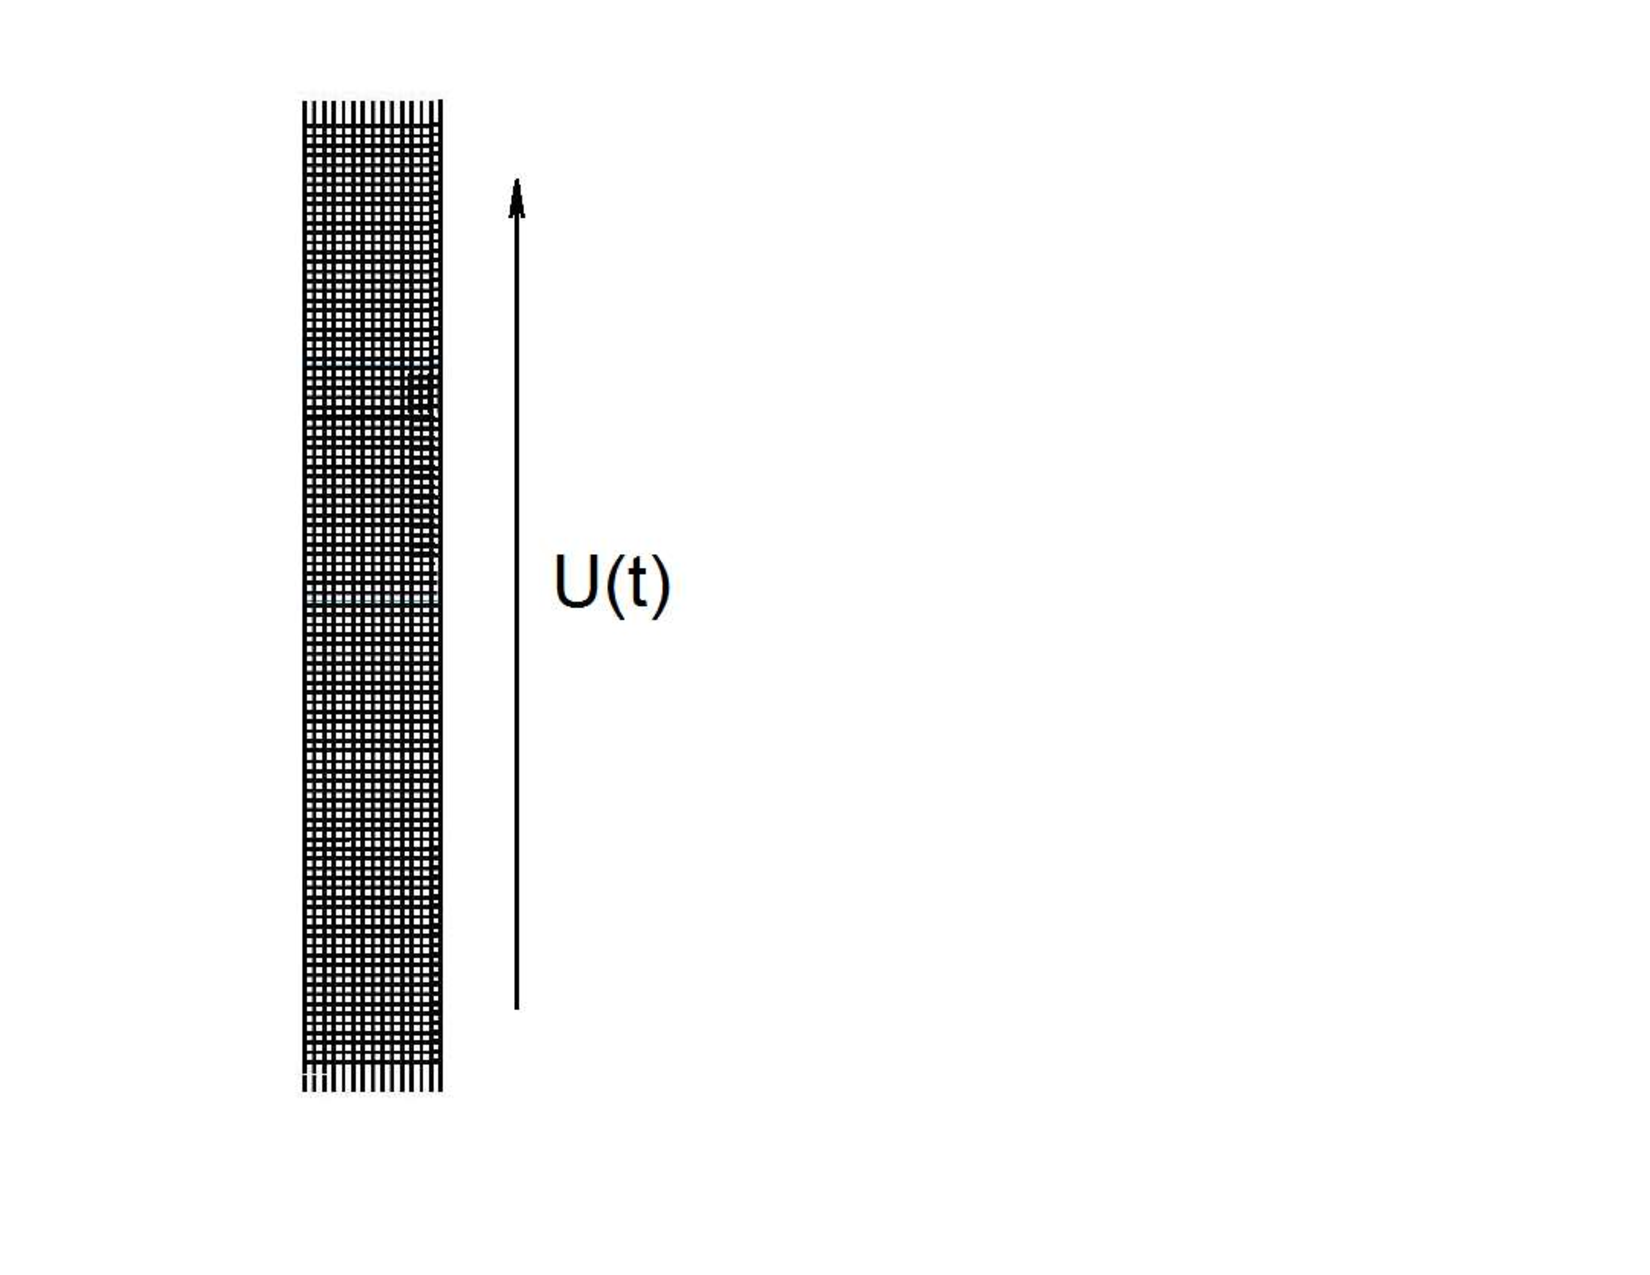
\includegraphics[scale=.3]{pictures/grid-minus1}
\caption{Schematic illustration of a quantum circuit for the time-evolution operator $U(t).$}.
\label{grid-0}
\end{center}
\end{figure}

Let $U_N(t)$ be the time evolution operator we are interested in, and let $t_*=\log N$ be the scrambling time in some units. Corresponding to $t_*$, one defines the unitary time evolution operator $V_N = U_N(t_*) = \exp(-iHt_*)$. Basically, we use $V_N$ to evolve into equilibrium state. In circuit representation, $V_N$ would have $K$ inputs and $K$ outputs (Question - This is due to unitarity, right?).

\begin{figure}[H]
\begin{center}
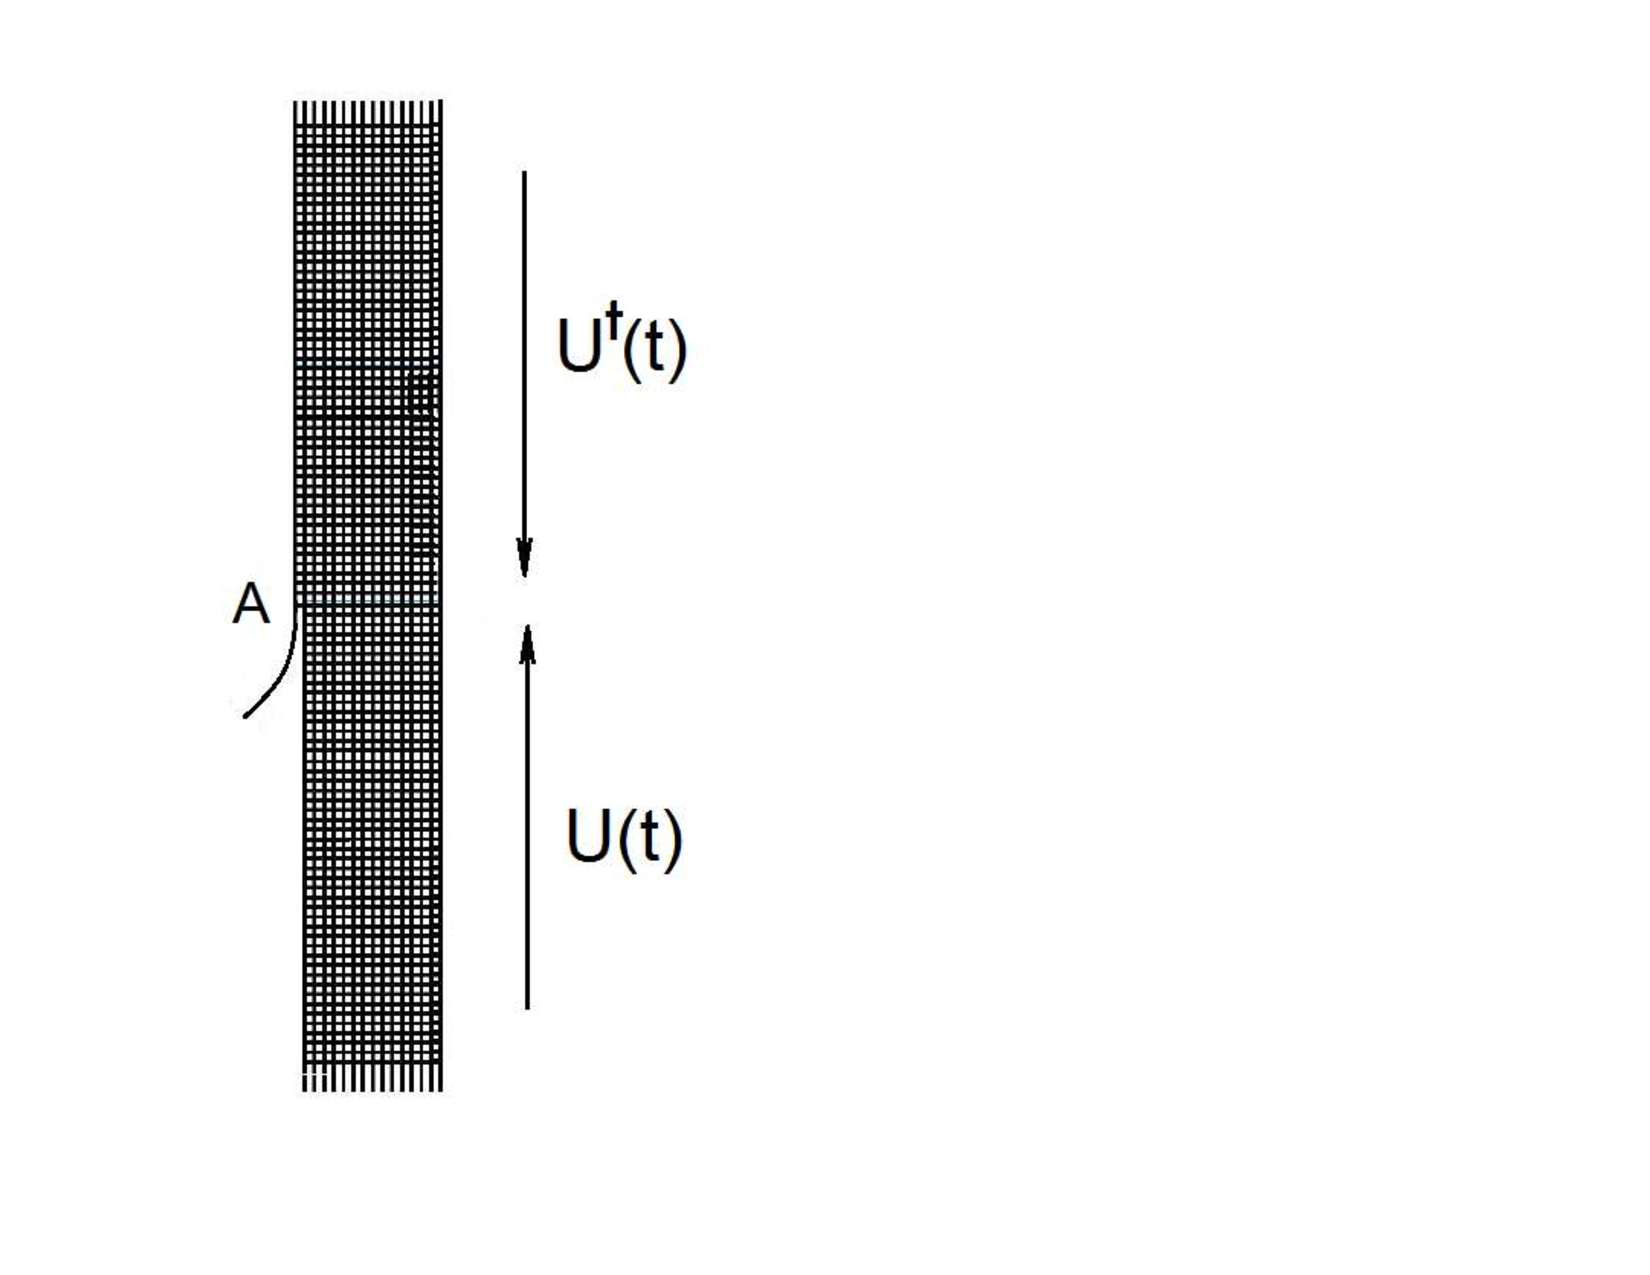
\includegraphics[scale=.3]{pictures/grid-0}
\caption{Time evolution operator for a precursor $U^{\dag}(t) \  A \ U(t)$ Note that the operator $U(t)$ acts on $N$ qubits and $U^{\dag}(t)$ acts on $N+1$ qubits.  The arrows on the right indicate the direction of time-flow.}
\label{grid-0}
\end{center}
\end{figure}

We would like to calculate the complexity of the teleportation protocol. This behooves us to define the notion of \textbf{complexity} in quantum computation. First, we define the size $s(t)$ of a one qubit operator $W$. $$s(t)= \sum_i \textbf{Tr}[W(t),X_i]^2$$ where $\textbf{Tr}$ denotes the normalized trace, i.e., $\bf Tr \it  I = 1$.

The size of a precursor grows exponentially with time until it saturates at the scrambling time,
\bea  
s(t)\eq e^t   \ \ \ \ \ t \leq t_*  \cr 
s(t) \eq N  \ \  \ \ \ t \geq t_*
\eea
The complexity of a precursor is related to the size by,
\be 
 \frac{\d\CC }{dt} = s(t).
\ee

Hence, for time scales lesser than $t_*$, $s$ and $\CC$ are essentially the same. The fact that complexity does not begin to grow linearly before the scrambling time is known as the \textbf{switchback effect}. This is related to the cancellation between the gates of $U$ and $U^{\dag}$. (Question - What exactly is this?)

For the circuit $V$, $\CC(V) = N \log N$. Hence for the time evolution $V^\dag \ W \ V$
\be 
\CC(V^{\dag} W V) \leq \CC(V^{\dag}) + \CC( W) + \CC( V) \approx 2N \log{N}.
\label{subadditivity}
\ee

But, the switchback effect says that $$\CC(V^{\dag} W V) \leq \CC(V^{\dag}) + \CC( W) + \CC( V) = N $$

\section{Teleportation Protocol}

Let us set up our quantum teleportation in the following manner :- 

\begin{itemize}
 \item Two mediating entangled systems belonging to Alice and Bob. Alice's portion of the mediator is called \textbf{A}, and Bob's is called \textbf{B}. This system is called the \textit{mediator}.
 \item Another system that Alice wishes to teleport to Bob. This system is denoted by \textbf{T}, and is called the \textit{teleportee}.
\end{itemize}

The entanglement entropy of the mediator is $N$. One can model such a system by considering $2N$ qubits in maximally entangled state. (Question - Why?)The teleportee is modelled as a system of $n$ qubits in the state $|\phi \ra$. The teleportation would be said to be \textit{successful} if a $n$-qubit subsystem of \textbf{B} becomes a pure state $|\phi \ra$.

There are a few things we would expect from teleportation :-
\begin{itemize}
 \item A successful teleportation diminishes the amount of entanglement by at least $n$. Hence $n \le N$ should be satisfied.
 \item Teleportation of $n$-qubit system requires transferring at least $2n$ classical bits between Alice and Bob. The classical transfer takes place through \textit{exterior} spacetime. (Question - What?! Why? How?)
\end{itemize}
 
In this protocol, we only consider small system teleportation, meaning $n<<N$. It is also imperative to define the notion of a computational basis for the teleportation, which is essentially the collection of simultaneous eigenvectors of the N (spin-flip) Pauli operators $Z_i$. We can label any state as $|I \ra = |11 \dots 010101 \ra$.

Let the initial state of the mediator be maximally entangled in the \textit{Thermofield Double state} (Question - What is this?) $$|TFD \ra = \sum_I |I \ra_A |I \ra_B$$ We also consider the teleportee to be in a state $|\phi \ra_T = \sum_k \phi(k) |k \ra_T$, where $k$ is the set of computational states in the Hilbert space of \textbf{T}. We can hence write the composite initial state as $$|initial \ra = \sum_{k,I} \phi(k) |k \ra_T |I \ra_A |I \ra_B  $$ Finally, we want there to exist a subsystem of Bob's qubits in the pure state $|\phi \ra_B = \sum_j \phi(j) |j \ra_B$

We shall assume that before teleportation begins, $\textbf{T}$ is absorbed and scrambled with the black hole degrees of freedom. This means we can be ready for teleportation only after $t_* = \log N$. In the initial state then, we combine Alice's mediator with the teleportee qubit to create $|AT \ra$ and scramble them together. Hence, we can write $$V|initial \ra = \sum_{k,I} \phi (k)V_{N+1} |kI \ra_{AT} |I \ra_B $$

We pick any two qubits from the $|AT \ra$ system and call them $\theta$. $\theta$ actually can stand for the following :-
\begin{itemize}
 \item The two chosen qubits.
 \item In the form $|\theta \ra$, basis states for the two-qubit system in the computational basis.
 \item A bit string of length two representing the outcome of an experiment of the two qubits.
\end{itemize}

The remaining $(N-1)$ qubits are denoted by $\alpha$. Hence, we can rewrite the above equation as 
$$V|initial \ra = \sum_{k,I,\theta,\alpha} \phi (k)|\theta,\alpha \ra \la \theta,\alpha| V_{(N+1)} |kI \ra_{AT} |I \ra_B
&=& \sum_{k,I,\theta,\alpha} \phi (k) V^{\theta,\alpha}_{k,I} |\theta,\alpha \ra |I \ra_B $$

Alice measures $\theta$ and gets some result. She sends this result in form of a classical two-bit string to Bob. Bob, on receiving the message, acts on his mediator subsystem with a unitary $Z^\theta$, The final state is hence,
$$\sum_{k,I,\theta,\alpha,j} \phi (k) V^{\theta,\alpha}_{k,I} |\theta,\alpha \ra \la \beta,j|Z^\theta|I \ra_B |\beta,j\ra_B$$
Here Bob's qubits have been partitioned to $(N-1)$ qubits named $\beta$ and one named $j$. This can be drawn as a circuit in the following way \newpage

\begin{figure}[H]
\begin{center}
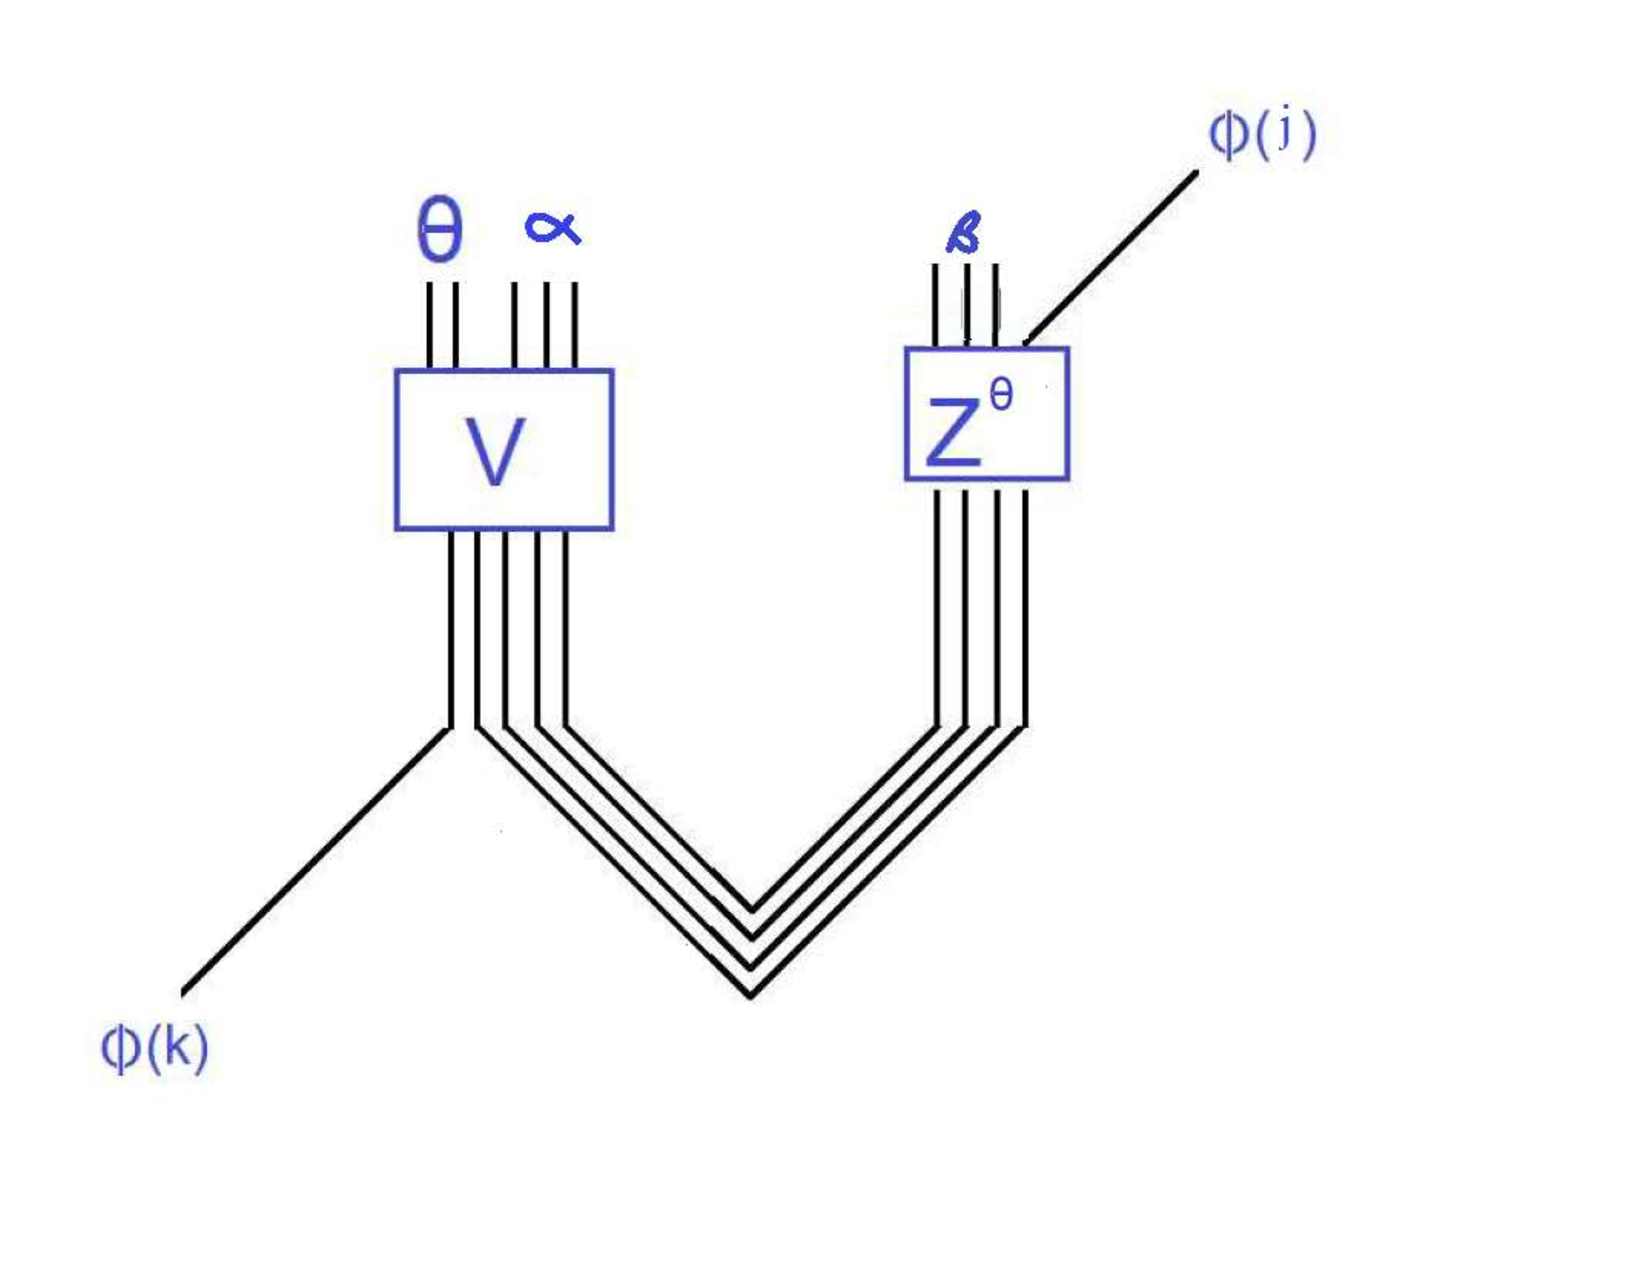
\includegraphics[scale=.3]{pictures/small-teleportation.pdf}
\caption{A circuit for teleporting a single qubit through an entangled state of $N+N$ qubits.  At this stage the unitary operator  $Z$ on Bob's side is unspecified}
\label{small-teleportation}
\end{center}
\end{figure}

\end{document}